\textit{This part of the thesis shows an extension of the previous work\cite{valdestilhasdbpediasameas} and cover the RQ5, in which we discuss the importance of the links for the Linked Data Web as they make a large number of tasks possible, including  cross-ontology, question answering and federated queries. However, a large number of these links are erroneous and can thus lead to these applications producing absurd results. We present a time-efficient and complete approach for the detection of erroneous links for properties that are transitive.
To this end, we make use of the semantics of URIs on the Data Web and combine it with an efficient graph partitioning algorithm. 
We then apply our algorithm to the LinkLion repository and show that we can analyze 19,200,114 links in 4.6 minutes. Our results show that at least $13\%$ of the \texttt{owl:sameAs} links we considered are erroneous. In addition, our analysis of the  provenance of links allows discovering agents and knowledge bases that commonly display poor linking.
Our algorithm can be easily executed in parallel and on a GPU. We show that these implementations are up to two orders of magnitude faster than classical reasoners and a non-parallel implementation.}

\subsection{The CEDAL approach}
%\todo[inline]{Main differences with previous version of CEDAL:(1)more Linksets (Lustre) (2) more properties (not only \texttt{owl:sameAs}, now also with \texttt{skos:exactMatch})}
Links across knowledge bases play a fundamental role in Linked Data~\cite{Albertoni:2013:ALQ:2457317.2457327} as they  allow users to navigate across datasets, integrate Linked Data sources~\cite{NgomoSL14}, perform federated queries~\cite{saleem2013daw} across data sources and perform large-scale inference on the data.
Given the importance of links, corresponding repositories such as \emph{sameas.org}\footnote{Link to the official web site: \url{http://sameas.org/}} and LinkLion~\cite{nentwig2014linklion} (of which \emph{sameas.org} is a subset) have been created. 
In addition to facilitating the finding of links between  resources and knowledge bases, these repositories also allow detecting significant errors across links. 
For example, according to LinkLion and by virtue of transitivity, the resources \texttt{orca:21075} and \texttt{orca:1946}\footnote{\texttt{orca} stands for the namespace \texttt{http://orca.cf.ac.uk/id/eprint/}.} stand for the same entity of the real world but have different URIs within the same knowledge base. 
This clearly goes against the definition of URIs as used in RDF. 
figure \ref{fig:example} shows a fictional example to help illustrate such problems, which can be classified as \textbf{contradiction problems}, according to the quality dimension of consistency~\cite{zaveri2015quality}. 
In our example, we can infer that one of the links along the path that led to this inference is wrong or that the knowledge base in itself contains an error. 
While such errors can be potentially detected by computing the closure of equivalence links using the characteristics of equivalence relations and an inference engine, our experiments with Pellet~\cite{bockbenchmarking} -- the fastest inference engine to the best of our knowledge -- suggest that inference engines do not scale to the millions of links found on the Web of Data. 

\begin{figure}[htb] 
	\centering
	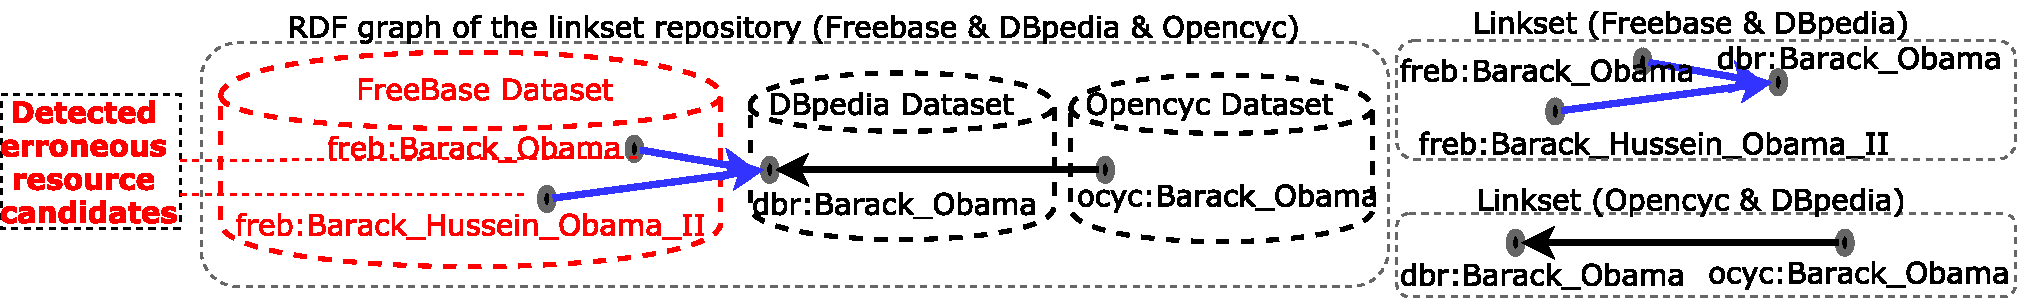
\includegraphics[width=1.0\linewidth]{img/example8.pdf}
	\caption{Manual detection of erroneous resource candidates.}
	\label{fig:example}
\end{figure} 

The poor performance on closure computations is also known from literature (see, e.g., ~\cite{arenas2008extension}). For instance, the computation of closures in RDF graphs has several drawbacks. Firstly, it is known that the \textbf{size} of the transitive closure of a graph $G$ is of \textbf{quadratic order} in the worst case, making the computation and storage of the closure too expensive for web-scale applications. Secondly, once the transitive closure has been computed, all queries are evaluated over a data source which can be much larger than the original one. This can be particularly \textbf{inefficient for queries} that must scan a large part of the input data.

Our intuition is that it is actually not necessary to compute the closures; instead, we can use adjacency lists and create graph partitions based on an algorithm called \emph{Union Find}~\cite{Tarjan:1975:EGB:321879.321884}. Therewith, we obtain a solution with a time complexity that is decreased from $O(n^2)$ to $O(m~log~n)$, where $m$ is the number of operations (either \emph{Union} or \emph{Find}) that are applied to $n$ elements.

In this paper, we aim to find erroneous links across knowledge bases by reusing the uniqueness of the semantics of URIs within given knowledge bases. We hence present a novel time-efficient algorithm called \textit{Consistency Error Detection Algorithm} \ac{CEDAL}, in which the error detection consists of finding distinct resources (i.e., resources with distinct URIs) which share the same dataset, given an RDF graph representing the union of all knowledge bases in a link repository.

With our work, we address the following research questions:
\begin{enumerate}
	\item Is there a time-efficient algorithm to detect erroneous links in large-scale link repositories?
	%\item Is there an efficient approach to automatically discover whether a linkset is coherent/consistent ?
	\item Is there an approach to discover whether a linkset\footnote{We refer to the definition of linkset as defined in the W3C document at \url{https://www.w3.org/TR/void/}.} is consistent without computing all closures required by the property axiom?
\end{enumerate}
%
The contributions of this work are listed below:
\begin{itemize}
	\item A time-efficient algorithm for the detection of erroneous links in large-scale link repositories without computing all closures required by the property axiom.
	\item An approach that brings the possibility to track the consistency problems inside link repositories.
	\item A scalable algorithm that works well in a parallel and non-parallel mode.
	\item A study case applied to a link repository called LinkLion.
	\item A new linkset quality measure based on the number of erroneous candidates.
\end{itemize} 
%
The remainder of this chapter is structured as follows: section \ref{approach} presents our algorithm for the detection of erroneous links in large-scale link repositories; section \ref{sessionErrorQuality} presents the error types and a quality measure for linksets; section \ref{ev:cedal} presents the evaluation of our approach.

\subsection{Method} \label{approach}
After introducing the terminology and symbolism used in this work, in this section, we present our error detection algorithm.
%to find whether two or more resources, inside the partition clusters, belong to the same dataset. 

\subsubsection{Error Detection algorithm}

Our algorithm targets consistency errors in large-scale link repositories. We assume a union of linksets $\mathcal{L}$ as given input. The aim is to find cases in which equivalent resources (according to the OWL semantics) in $\mathcal{L}$ share the same dataset. The basic intuition here is equivalent resources (i.e., resources that stand for the same entity from the real world) being in one knowledge base is a clear hint towards (1) an error in the knowledge base itself or (2) an error during the generation of the links that allowed generating this equivalence.

%A focus of our algorithm is the quality dimension of consistency, applied to large scale link repositories in order to find cases in which given a union of homogeneous knowledge bases $L$, find in $L$ equivalent resources that share the same dataset.

%of \textit{two or more equivalent objects with different identifiers}, but inside the same link-set that also belongs to the same dataset.

In figure \ref{fig:ErrorDetection}, we show how our algorithm works. Given datasets $D_1,...,D_n$, resources $R=\{a,b,c,d,e,f\}$, the idea is to detect two or more resources sharing the same dataset inside the same cluster, following the steps described in the following list and into the algorithm \ref{alg:err}.

\begin{enumerate}
	\item As input, the algorithm receives a set of linksets $L=\{(r_1,r_2),...,(r_n,r_m)\}$, where $r_n$ represents the resources.
	\item The linksets are merged creating a unique RDF graph $\mathcal{L}= \bigcup_i L_i$, where $L_i={(s,p,o):s \in D_i^{(s)}, o \in D_i^{(t)}}$, $D$ represents source and target datasets of the linksets and $(s,p,o)$ are subject, predicate and object of an RDF triple.
	\item From $\mathcal{L}$, create clusters $\mathcal{C}$, containing the resources, datasets and the knowledge base.
	\item Find cases in which two or more resources $r_i$ belong to the same dataset $D$.
	\item Put these resources, related paths, dataset names and knowledge-bases into a list and return this list $\mathcal{O}$. %\todo{TS: Try to present the theoretical point of view. ``Putting stuff into a list'' is already part of the implementation. You can comment this, but do mention $\mathcal{O}$ below as the output.}
	\item The output are all paths that were considered wrong and the original mappings.
\end{enumerate}

Our algorithm works by partitioning a graph inside an adjacency list that contains: (1) An array per vertex for a total of $V$ arrays, where we are only considering the space for the array pointer, not the contents of the array. (2) Each directed edge is contained once somewhere in the adjacency list, for a total of $E$ edges, where a bidirectional edge is just $2$ directed edges, assuming we are using bi-directional edges. 

In this context we are using techniques from an well know algorithm called Union-Find, where the definition in computer science, is based in a disjoint-set data structure, also called a merge–find set, is a data structure that keeps track of a set of elements partitioned into a number of disjoint (non overlapping) subsets. It supports two useful operations:

(1)Find: Determine which subset a particular element is in. Find typically returns an item from this set that serves as its "representative"; by comparing the result of two Find operations, one can determine whether two elements are in the same subset.

(2)Union: Join two subsets into a single subset.


% Thus, we have $V+E$ therefore, $O(V + E)$, about computational time complexity. 

%\todo{TS: Multiple issues at this point: (1) Remove ``if we are using bidirectional edges'' and assume that they can exist. (2) What is ``it'' in ``it would just be $2E$? (3) If we are talking about computational time complexity, let's say it.}

\begin{figure}[htb] 
	\centering
	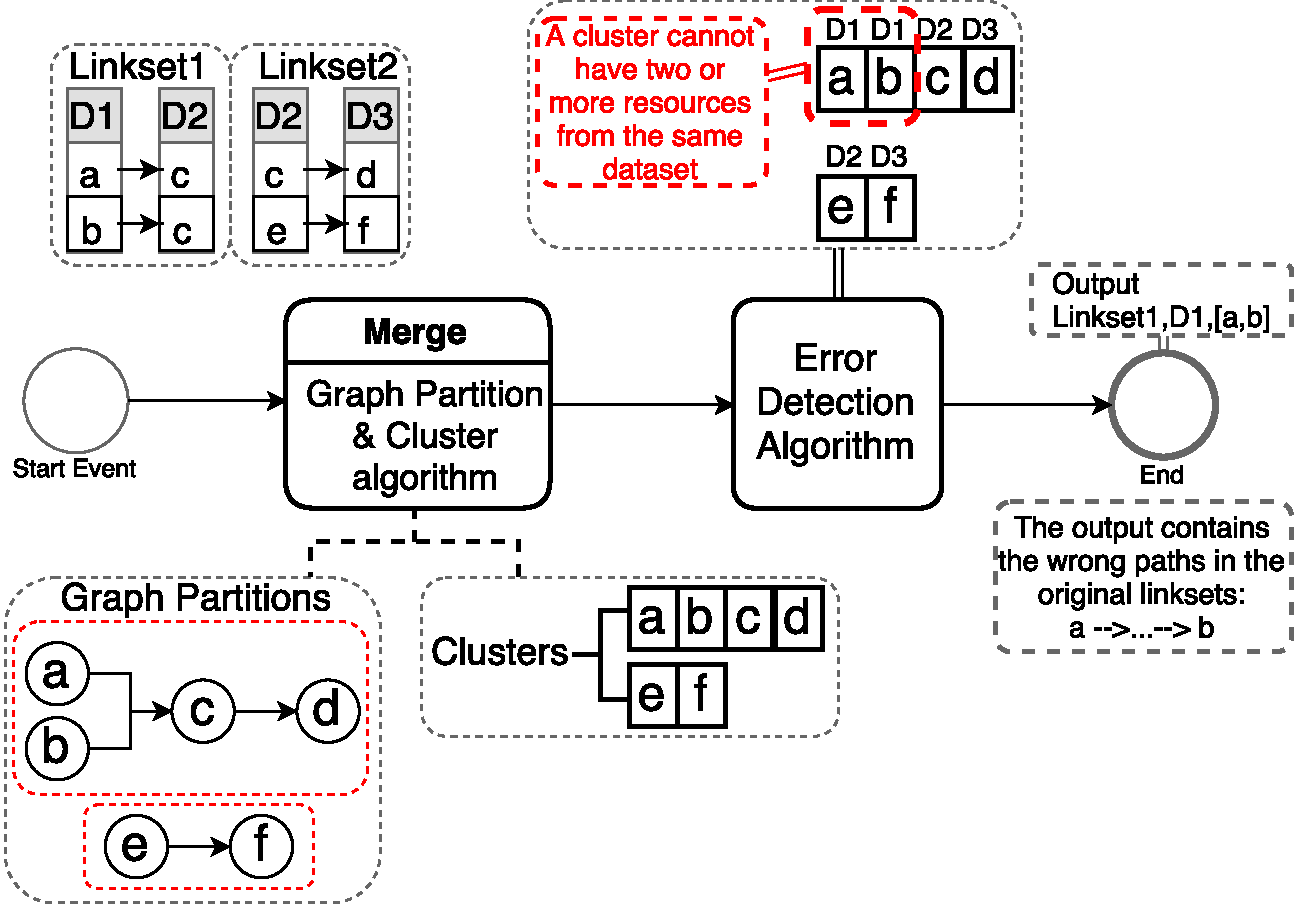
\includegraphics[width=0.86\linewidth]{img/errorDetection8.pdf}
	\caption{Error detection.}
	\label{fig:ErrorDetection}
\end{figure} 

%\begin{algorithm} [hbt]  
%	\caption{Error detection algorithm}
%	\label{alg:err}
%	%\begin{algorithmic}[1]
%	\textbf{Input}: An Graph $G(V,E)$ already with the closures (Reflexive, Symmetric and Transitive) \\
%	\textbf{Output}: An error list with erroneous nodes.
%	\begin{algorithmic}[1]
%		\Procedure{ErrorDetection($G(V,E)$)}{}
%		\State{push $G(V,E)$ onto cluster relating nodes with his datasets}
%		
%		\If{A cluster has more than one node from the same dataset}
%		\State{push the these nodes and respect edges onto a Error List}
%		\EndIf
%		\State{Write the Error List}
%		\EndProcedure
%	\end{algorithmic}
%	%\end{algorithmic}
%\end{algorithm}

\begin{algorithm} [htb] 
	\caption{Consistency Error Detection Algorithm (CEDAL)}
	\label{alg:err}
	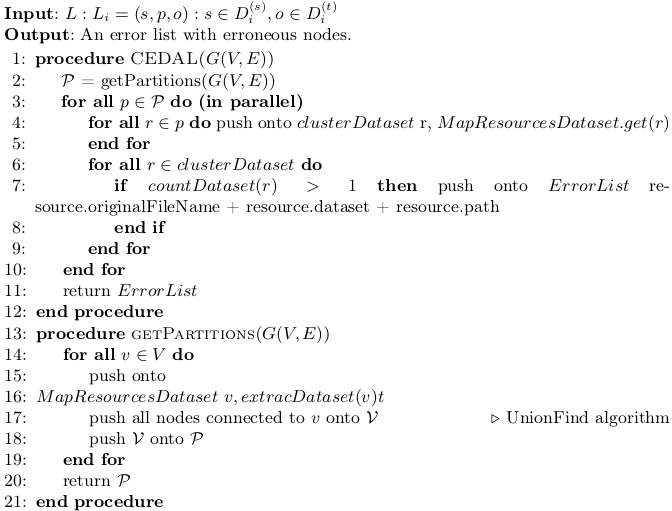
\includegraphics[width=\linewidth]{sections/img/algCedal.png}
\end{algorithm}

\subsubsection{Problem statement.}
We formalize the problem of \textit{detection of erroneous links in large-scale link repositories} as follows.

%Using the symbols from table \ref{tab:symbols} we will formalize the problem. 

%\begin{table}[H]
%	\centering
%	\caption{Symbols}
%	\label{tab:symbols}
%	\begin{tabular}{llllllll}
%		$\mathcal{D}$   & Set of all datasets in $\mathcal{L}$  \\
%		$\mathcal{L}$     & Set of all linksets   \\
%		$D$   & a dataset                  \\
%		$L$ & a linkset                           \\
		%$\mathcal{L}^*$  & linksets with closures computed(Check if we are still using)   \\
%		$\mathcal{O}$ & Output with erroneus candidates \\ 
%		$\mathcal{C}$ & The clusters about the graph partitions   \\
%		$P$ & represents the path of resources with errors. \\
%		$s,p,o$ & subject, predicate, object.              
%	\end{tabular}
%\end{table}

From this section on, we will refer to the union of all linksets as $\mathcal{L} = \bigcup_i L_i$, the set of all datasets as $\mathcal{D}$, the clusters (or graph partitions) as $\mathcal{C}$, the candidates (i.e., set of resources belonging to the same dataset) $\mathcal{P}$.
A linkset $L \in \mathcal{L}$ contains triples (or links) $(s,p,o)$ such as:
\begin{equation} \label{eq:linkset}
(s,p,o) \in L : s \in D_i, o \in D_j, i \neq j
\end{equation}

% $\mathcal{P}$ contains candidates $P$ composed by links that belong to the equivalence closure $\mathcal{L}^*$ of $\mathcal{L}$.
Each candidate $P$ abides by the following restriction:
\begin{equation} \label{eq:cand} % P = \{r_1, \ldots, r_n\} \in \mathcal{P}
\forall r_i,r_j \in P : r_i \neq r_j \Rightarrow (r_i, x, r_j) \in \mathcal{L}^* \vee (r_j, x, r_i) \in \mathcal{L}^*
\end{equation}
where $x$ is a property (e.g., \texttt{owl:sameAs}).
In other words, each element in $P$ is linked to at least another element in the set.
Candidates are assigned one of two classes, positive (i.e., candidates with errors) or negative.
The positive cases are represented as follows.
\begin{equation} \label{eq:f1}
P \in \mathcal{P}^+ \iff \left(\exists r_1 \in P \cap D_1, r_2 \in P \cap D_2 \right) \therefore D_1 = D_2 \Rightarrow r_1 \neq r_2
\end{equation} 
% Here, the error was detected and the resources added to a list of error, that contains the path of the knowledge base file, the	dataset and the resources where the error was detected inside the cluster.
The negative cases are defined in the following equation.
\begin{equation} \label{eq:negativeF1}
P \in \mathcal{P}^- \iff \left(\forall r_1 \in P \cap D_1, r_2 \in P \cap D_2 \right) \therefore D_1 = D_2 \Rightarrow r_1 = r_2
\end{equation} 
% Finally, \cref{eq:output} represents the output with the path of the resources. 
The target is thus to find the set of erroneous candidates $\mathcal{P}^+$.
As shown in the next section, we cannot state that a link connecting these resources is wrong, but we can state that the error lies somewhere between the links that connect them and the organization of the dataset they belong to.

% \begin{equation} \label{eq:links}
% o = p(s) \iff (s,p,o) \in  \mathcal{L}^*
% \end{equation}

% \begin{equation} \label{eq:pairs}
% P_{s,o} = {p_1,..., p_k : p_k(...(p_1(s))) = o}
% \end{equation}

% \begin{equation} \label{eq:output}
% \mathcal{O} = P_{(r_1,r_2)}
% \end{equation}
%This brings the possibility to track the conciseness problems inside linkset repositories, such as LinkLion, because $\mathcal{O}$ contains the dump-file-name, the dataset-name and the path inside the cluster where the problem was detected.

%\begin{equation}
%\sum_{P \in \mathcal{P}^-} |P|-1
%\end{equation}

\subsection{Error Types and Quality Measure for Linkset Repositories} \label{sessionErrorQuality}

The application of the two measures requires the output from CEDAL, allowing to identify two types of errors among the erroneous candidates from the output.

%Based on CEDAL algorithm we present a new quality dimension evaluating the information accessed cross-walking the linksets of LinkLion. 
%To this purpose, we identify in the following formula:
%\begin{equation}
% CEDALQ=\frac{\sum \mu-1}{\sum_{P \in \mathcal{P}^-}|P|-1}
%\end{equation}
%Where $\mu$ represents the score and $P$ the output set carrying erroneous candidates.

\subsubsection{Error Types} \label{errorType}

%\todo[inline]{TS: The following text contains repetitions of text above. Although it's common in theses and books, this shouldn't happen in a paper. Remove the redundancies.}

%\todo{TS: Unfortunately, this is not true: ``Our algorithm is able to detect two types of errors''. We are able to identify them only manually! I'd replace it with ``We identified two types of errors which can be defined...''. Maybe explain why we cannot do that automatically.}

We identified two types of errors, in which can be defined in quality dimensions by~\cite{zaveri2015quality}. (1) \textbf{Semantic accuracy} errors, in which we detect if data values correctly represent the real world facts. (2) \textbf{Consistency} and \textbf{Conciseness} errors where a knowledge base is free of logical or formal contradictions concerning particular knowledge representation and inference mechanisms and the minimization of redundancy of entities at the schema and the data level. 
figure \ref{fig:errorType} shows a fictional example of both error types, in which we represent links between  GeoNames\footnote{Link to the official web site: \url{http://www.geonames.org/}} and DBpedia.\footnote{Link to the official web site: \url{http://dbpedia.org/}}
%We identified two types of errors, in which can be defined in quality dimensions by~\cite{zaveri2015quality}. (1) \textbf{Semantic Accuracy} errors, in which we detect if data values correctly represent the real-world facts. (2) \textbf{Consistency} errors where a knowledge base is free of (logical or formal) contradictions concerning particular knowledge representation and inference mechanisms. The figure \ref{fig:errorType} shows a fictional example of both of error types, in which we represent links between  GeoNames\footnote{\url{http://www.geonames.org/}} and DBpedia\footnote{\url{http://dbpedia.org/}}.
\begin{figure}[H]
	\centering
	\subfigure[Error type (1).] 
	{
		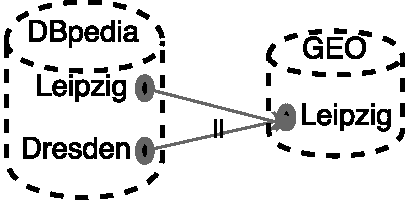
\includegraphics[width=0.4\linewidth]{img/CEDAL1_2.pdf}
		\label{fig:error1}
	}
	\subfigure[Error type (2).] 
	{
		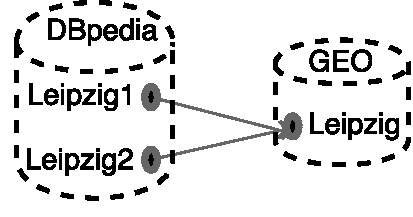
\includegraphics[width=0.4\linewidth]{img/CEDAL2_2.pdf}
		\label{fig:error2}
	}
	\caption{Detected error types.}
	\label{fig:errorType}
\end{figure}
%
In this example, figure \ref{fig:error1} shows an error of type (1), in which an erroneous \texttt{owl:sameAs} link between the city of Dresden and the city of Leipzig was detected. The figure \ref{fig:error2} shows an error of type (2) where the resource about the city of Leipzig is duplicated within the DBpedia dataset. 

We manually analyzed a random sample of the errors. Among $100$ occurrences, $90\%$ are of type (2). It was not feasible in practice to perform this evaluation in an automatic way, due to the fact that it involves semantic accuracy and thus needs human feedback. Moreover, some URIs are unreachable, resulting many times in \textit{timeout errors}, such as HTTP $404$, $500$ and $503$ errors.\footnote{Error types from W3c: \url{https://www.w3.org/Protocols/rfc2616/rfc2616-sec10.html}} In summary, it was not practicable to automatically distinguish these types of errors among the erroneous candidates detected by CEDAL. % In other words, CEDAL detects automatically erroneous candidates, allowing manually identify error types(1 and 2) among the candidates.

\subsubsection{Quality Measure}

Based on the error types from CEDAL, we present three linkset quality measures, evaluating the information accessed by cross-walking the linksets of LinkLion.

The \textbf{Semantic Accuracy of linksets} indicates whether the data values from the RDF links represent real world facts.
\textbf{Example:} Let us assume that we have a linkset from DBpedia and Geonames. A link \texttt{<dbr:dresden owl:sameAs geo:leipzig>} would clearly be inaccurate, since Dresden and Leipzig are two different cities.

The \textbf{consistency and conciseness of links} inform whether a linkset is free of logical or formal contradictions with respect to particular knowledge representation and inference mechanisms and the minimization of redundancy of resources that belongs to the same dataset inside a linkset repository.
\textbf{Example:} With a linkset from DBpedia and Geonames, let us assume we found two links represented by \texttt{<dbr:leipzig1 owl:sameAs geo:leipzig>} and \texttt{<dbr:leipzig2 owl:sameAs geo:leipzig>}. Since \texttt{dbr:leipzig1} and \texttt{dbr:leipzig2} belong to the same dataset, this characterizes a redundancy and it contradicts the assumption that two URIs in a dataset cannot stand for the same thing from the real world.

%\todo{You say two metrics at the beginning of this section, now we have three. No equations for M2 and M3, ergo unclear how to compute them. Please clarify.}
In order to evaluate data quality in linksets, on the lines of the works summarized in the Data Quality survey~\cite{zaveri2015quality}, we propose three new metrics:
\begin{description}
\item[M1:] Rate of consistent resources inside linkset repositories.

Let us consider a candidate $P \in \mathcal{P}$ containing only resources which belong to the same dataset. The rate of consistent candidates is defined as follows:
\begin{equation} \label{eqn:m1}
M1=\frac{ \sum_{P \in \mathcal{P}^-} |P|}{ \sum_{P \in \mathcal{P}} |P|}
\end{equation}
where $\mathcal{P}^-$ is the set of consistent (i.e., non-erroneous) candidates. We call $M1$ the \textbf{consistency index}.
%Shall we normalize [0,1] ?: $\frac{X-\min(X)}{\max(X)-\min(X)}$
\item[M2:] Rate of candidates in $\mathcal{P}$ containing resources whose internal links are real world facts. Let us introduce a function $f(s,p,o)$ which expresses the verification of a triple $(s,p,o)$ in the real world, assuming value $1$ if the statements holds true and $0$ otherwise. This metric addresses errors of type (1).
\end{description}
%
\begin{equation}
M2= \frac{ | \{ P \in \mathcal{P}^+ : \forall r_i, r_j \in P \ r_i \neq r_j \Rightarrow f(r_i, p, r_j) = 1 \} | + |\mathcal{P}^-| }{ |\mathcal{P}|  }
\end{equation}
%
\begin{description}
\item[M3:] Rate of candidates in $\mathcal{P}$ which are free of redundant resources. This metric addresses errors of type (2).
\end{description}
%
\begin{equation}
M3= \frac{ | \{ P \in \mathcal{P}^+ : \exists r_i, r_j \in P \ r_i \neq r_j \Rightarrow f(r_i, p, r_j) = 0 \} | + |\mathcal{P}^-| }{ |\mathcal{P}|  }
\end{equation}
%
As can be seen, M2 and M3 are dependent on each other.

In this paper, we focus on the computation of M1. 
Although M2 and M3 are left for future research, we included them to encourage their evaluation and use.

%Was possible to define these metrics thanks to the work~\cite{zaveri2015quality}
%This metrics was only possible because we use as base the 

\subsection{Evaluation} \label{ev:cedal}

To verify our hypothesis, in this section we show that CEDAL brings an efficient way to track the erroneous candidates inside large-scale linkset repositories. 

\subsection{Experimental setup}
As our study case, we use a linkset repository called LinkLion~\cite{nentwig2014linklion} due to some advantages such as provenance, linksets from the most used datasets, i.e. DBpedia, Yago and Opencyc, where the users are empowered to upload links and specify how these were created. Moreover, users and applications can select and download sets of links via dumps or SPARQL queries. 

The table \ref{tab:linkTypes} shows that $99.9 \%$ of links from LinkLion are \texttt{owl:sameAs} links, amounting to $19,200,114$ triples. Thus, in our experiments we are using only \texttt{owl:sameAs} links. 
% All linkset files from LinkLion were copied locally to run the experiments.

\begin{table}[H]
	\centering
	\caption{Link types}
	\label{tab:linkTypes}
	\begin{tabular}{ll}
		\hline\noalign{\smallskip}
		\textbf{Property}   & \textbf{Triples}  \\
		\noalign{\smallskip}
		\hline
		\textbf{sameAs}     & 19,606,657 (with duplicates)    \\
		\textbf{country}    & 1,309                 \\
		\textbf{author}     & 766              \\
		\textbf{spokenIn}   & 624                  \\
		\textbf{locatedIn}  & 250                  \\
		\textbf{exactMatch} & 167                 \\
		\textbf{near}       & 30                   \\
		\textbf{spatial\#P} & 28                   \\
		\textbf{seeAlso}    & 14             \\
		\textbf{organism}   & 14      \\
		\textbf{made}       & 4                \\
		\hline           
	\end{tabular}
\end{table}
%
The experiments were performed using two configurations: (1) a laptop with Intel Core i7, 8 GB RAM, a video card NVIDIA NVS4200, Operational System MS Windows 10 and Java SE Development Kit 8. (2) An Intel Xeon Core i7 processor with 40 cores, 128 GB RAM on an Ubuntu 14.04.5 LTS with Java SE Development Kit 8. The results including the output file for LinkLion are available online.
The total number of $19.6 million$ links was processed by our algorithm in $4.6$ minutes with the configuration (2). The total amount of errors were $1,352,366$ of candidates, where the total amount of domains were $254$ and  the number of linkset files was $553$, where $48.3\%$ of these knowledge base files has less than $10$ resources detected as erroneous candidates. 

\subsubsection{Ranking the erroneous candidates}
%Our ultimate goal is to detect links in \textit{large-scale link repositories}, resources sharing the same dataset.
To evaluate how effective CEDAL is, we create a score in order to rank the erroneous candidates based on the number of detected resources with errors, in which the table \ref{tab:tuples}, show two fictional examples of tuples in the same pattern of the output from CEDAL.

\begin{table}[H]
	\centering
	\caption{Fictional example results.}
	\label{tab:tuples}
	\begin{tabular}{@{}llll@{}}
		\toprule
		Knowledge-base & Data-set domain & \textbf{$\mathbb{C}$} & $\mu$ \\ \midrule
		Linkset1.nt                 & Data-set1         & URI1,URI2               & 1              \\
		Linkset2.nt                 & Data-set2         & {\small URI1,URI2,URI3,URI4}     & 6              \\ \bottomrule
	\end{tabular}
\end{table}
%
The $\mu$ score is calculated by $\mu = \frac{|\mathbb{C}|(|\mathbb{C}| - 1)}{2}$, in which we use the cardinality of $\mathbb{C}$ representing the detected erroneous candidates. The figures \ref{fig:ErrorCounts} and \ref{fig:a2} shows the top 5 erroneous candidates according to the rank score.

\newcommand{\slice}[4]{
  \pgfmathparse{0.5*#1+0.5*#2}
  \let\midangle\pgfmathresult

  % slice
  \draw[thick,fill=black!10] (0,0) -- (#1:1) arc (#1:#2:1) -- cycle;

  % outer label
  \node[label=\midangle:#4] at (\midangle:1) {};

  % inner label
  \pgfmathparse{min((#2-#1-10)/110*(-0.3),0)}
  \let\temp\pgfmathresult
  \pgfmathparse{max(\temp,-0.5) + 0.8}
  \let\innerpos\pgfmathresult
  \node at (\midangle:\innerpos) {#3};
}

\begin{figure}[htb]
	\centering
	\subfigure[Top 5 Knowledge-base pairs with more candidates.]
	{
		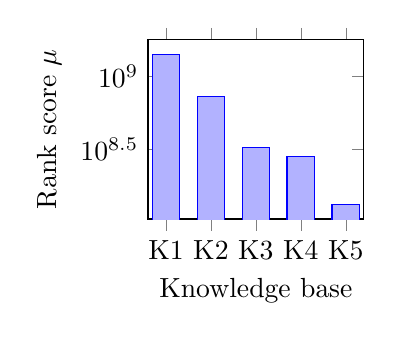
\begin{tikzpicture}
		\begin{axis}[
		scale=0.40,
		ymode = log,
		ybar,
		xlabel={Knowledge base},
		ylabel={Rank score $\mu$},
		symbolic x coords={K1,K2,K3,K4,K5},
		xtick=data,
		]
		\addplot coordinates { (K1,1408398201)(K2,728111880)(K3,325520370)(K4,284137041)(K5,133882066)};
		\end{axis}
		\end{tikzpicture}
		\label{fig:a1}
	}
	\subfigure[Top 5 Knowledge-base pairs with fewer candidates.]
	{
		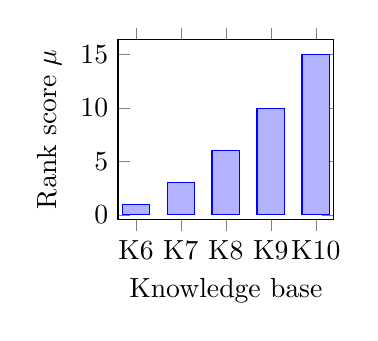
\begin{tikzpicture}
		\begin{axis}[
		scale=0.40,
		ybar,
		xlabel={Knowledge base},
		ylabel={Rank score $\mu$},
		symbolic x coords={K6,K7,K8,K9,K10},
		xtick=data,
		]
		\addplot coordinates { (K6,1)(K7,3)(K8,6)(K9,10)(K10,15)};
		\end{axis}
		\end{tikzpicture}
		\label{fig:a2}
	}
	\subfigure[input size=$10^3$.] 
	{
		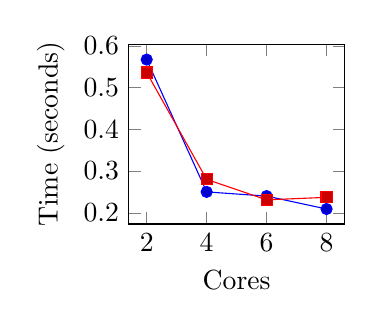
\begin{tikzpicture}
		\begin{axis}[
		scale=0.40,
		%ymode = log,
		legend style={legend pos=outer north east,font=\tiny},
		xlabel=Cores,
		ylabel=Time (seconds)
		]
		\addplot coordinates { % GPU
			(2,0.567) (4,0.25) (6,0.24) (8,0.209)
		};
		\addplot coordinates { % CPU
			(2,0.536) (4,0.280) (6,0.231) (8,0.237)
		};
		%\legend{
		%	GPU,
		%	CPU
		%}
		\end{axis}
		\end{tikzpicture}
		\label{fig:r2}
	}
	\subfigure[input size=$10^6$.] 
	{
		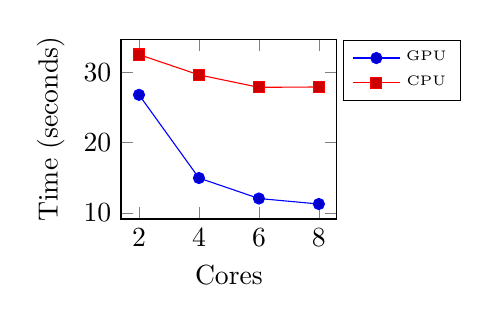
\begin{tikzpicture}
		\begin{axis}[
		scale=0.40,
		%ymode = log,
		legend style={legend pos=outer north east,font=\tiny},
		xlabel=Cores,
		ylabel=Time (seconds)
		]
		\addplot coordinates { % GPU
			(2,26.776) (4,14.947) (6,12.034) (8,11.251)
		};
		\addplot coordinates { % CPU
			(2,32.500) (4,29.613) (6,27.844) (8,27.891)
		};
		\legend{
			GPU,
			CPU
		}
		\end{axis}
		\end{tikzpicture}
		\label{fig:r3}
	}
	\caption{Error rank (legends: see table \ref{tab:legends}) and 
	Runtime results according to the input size, CPU and GPU.}
	\label{fig:ErrorCounts}
\end{figure}

\begin{table}[H]
	\small
	\centering
	\caption{Legend for the figures \ref{fig:ErrorCounts} and \ref{fig:a2}}
	\label{tab:legends}
	\begin{tabular}{@{}llll@{}}
		\toprule
		Label & Knowledge Base  \\ \midrule
		K1  & dotac.rkbexplorer.com---eprints.rkbexplorer.com.nt      \\
		K2  & d-nb.info---viaf.org.nt                                \\
		K3 & dblp.rkbexplorer.com---dblp.l3s.de.nt                    \\
		K4 & linkedgeodata.org---sws.geonames.org.nt                 \\
		K5 & citeseer.rkbexplorer.com---kisti.rkbexplorer.com.nt     \\
		K6 & wiki.rkbexplorer.com---oai.rkbexplorer.com.nt            \\
		K7 & www4.wiwiss.fu-berlin.de---dbpedia.org.nt                \\
		K8 & southampton.rkbexplorer.com---nsf.rkbexplorer.com.nt    \\
		K9 & rae2001.rkbexplorer.com---newcastle.rkbexplorer.com.nt  \\
		K10 & lod.geospecies.org---bio2rdf.org.nt                    \\ \bottomrule
	\end{tabular}
\end{table}
%
%According to our rank, the knowledge-base with more errors comes from $periodicals.dataincubator.org$ with $93,584$ links per mapping\footnote{Links per mapping from \url{http://www.linklion.org/}}, in which we found $2,159$ erroneous resource candidates and a score of $2,329,561$. The knowledge base with fewer errors was $bio2rdf.org$ with $340,468$ links per mapping, in which we found $2$ erroneous resource candidates and a score of $1$, also $193$ datasets with no errors at all.
%\todo{Fix this, according the table and fill out the table.}

Considering only linksets between different datasets, the knowledge-base with more errors comes from the links in
\begin{verbatim}
    dotac.rkbexplorer.com - eprints.rkbexplorer.com
\end{verbatim}
with $458,324$ links per mapping\footnote{Links per mapping from \url{http://www.linklion.org/}}, in which we found $53,074$ erroneous resource candidates resulting in a score of $1,408,398,201$. The knowledge base with fewer errors comes from the links in
\begin{verbatim}
    lod.geospecies.org - bio2rdf.org.nt
\end{verbatim}
with $9,723$ links per mapping, in which we found $6$ erroneous resource candidates and a score of $15$, also $193$ datasets with no errors at all.

\subsubsection{Runtime experiments}

The experiments were performed with the input size varying between $10^3$ and $10^6$ RDF triples using the configuration (1), as shown in figures \ref{fig:r2} and \ref{fig:r3}. Our algorithm processed all $19,200,114$ links from LinkLion in $4.6$ minutes with the configuration (2). 
The results indicate that our algorithm scales well to large links repositories and can also be adapted to the hardware on which it is executed. For example, it can be easily implemented to make use of benefits of CPUs and GPUs.

\subsubsection{Scalability Evaluation}

Our algorithm performs well in parallel and non-parallel environments. The performance of our algorithm improved in accordance to the number of CPUs, showing that our algorithm is scalable, performing well with large linksets with size more than $10^6$ as shown in figures \ref{fig:r2} and \ref{fig:r3}.

\subsubsection{Parallel Implementation}

Our algorithm implementation contains parallel code snippets in which we perform a load-and-balance of the data among CPU/GPU cores when available. This specific characteristic offers the possibility for utilization when hardware for parallel computing is available, such as CPU/GPU processors.

%\todo[inline]{TS: The following paragraph is not necessary.}

To illustrate this part of our idea, we can state: Given a graph $G(V,E)$, that contains all linksets from the repository $G(V,E) \subseteq \mathcal{L}$, this graph has partitions $P \subset G(V,E)$. Thus, errors are calculated for each partition, the processes are separated in threads and these threads are spread among CPU/GPU cores. Thus, we process the graph partitions in parallel, as shown in figure \ref{fig:cpugpu1}.
%, according to the parallel processing as shown in figure \ref{fig:cpugpu2}.

\begin{figure}[H]
	\centering
	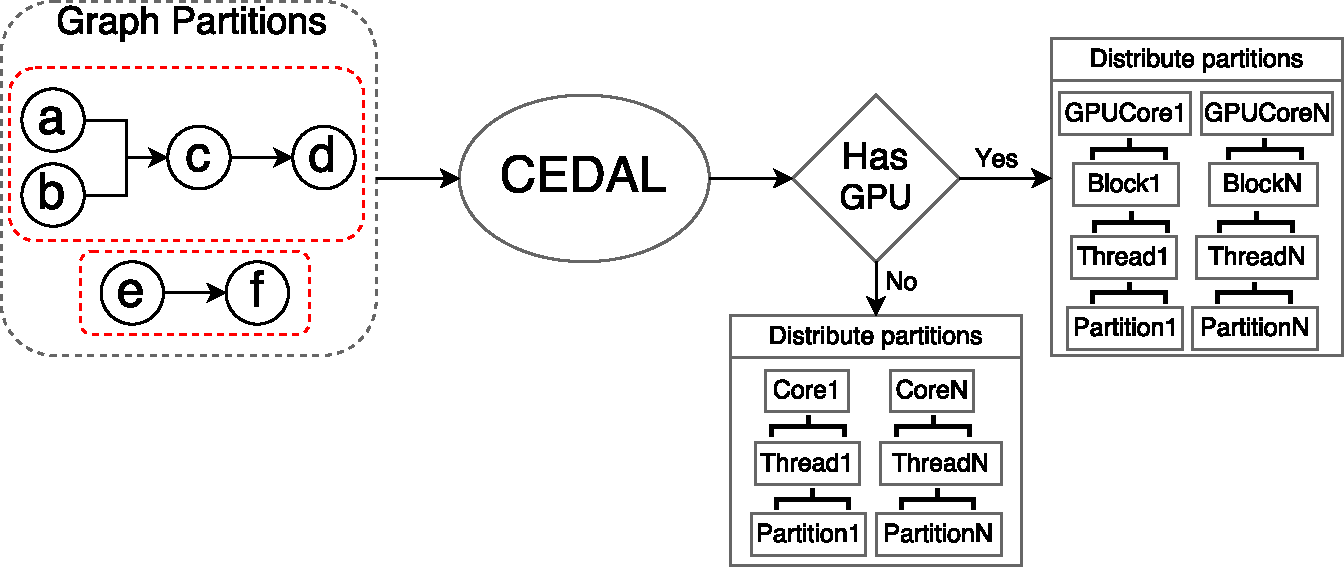
\includegraphics[width=0.9\linewidth]{img/cpugpu4.pdf}
	\caption{CEDAL CPU/GPU processing}
	\label{fig:cpugpu1}
\end{figure}

%\begin{figure}[H]
%	\centering
%	\includegraphics[width=0.7\linewidth]{img/cpugpu}
%	\caption{CPU/GPU processing~\cite{harish2007accelerating}}
%	\label{fig:cpugpu2}
%\end{figure}

\subsubsection{Consistency by provenance of links}
%\todo[inline]{TS: \textbf{Consistency by Provenance?}}
%\subsection{Consistency (Human vs Algorithms)}
%\subsection{Consistency (Framework )}
Thanks to the information found in LinkLion, we are able to check the provenance of links. This allowed us to analyze them more in details by finding which link discovery framework has created the link. The links were generated by four types of frameworks: \textit{LIMES}~\cite{ngomo2011limes}, \textit{SILK}~\cite{volz2009silk},  \textit{DBpedia Extraction Framework}~\cite{lehmann2015dbpedia} and \textit{sameas.org}\footnote{Link to the official web site: \url{http://sameas.org}}. The type of links provided by \textit{sameas.org} were generated into human-curated knowledge bases, such as DBpedia (which is based on Wikipedia), Freebase, and OpenCyc.

We found a $13.5\%$ error rate from \textit{sameas.org} versus a $4.1\%$ error rate of the algorithms such as \textit{LIMES}~\cite{ngomo2011limes}. They are all below $5\%$ as table \ref{tab:frameworks} shows; column $Errors$ represents the rate of all resources belonging to error candidates and column $M1$ represents the respective quality measure. 
% We calculate the percentage of error with a simple formula $\% = \frac{Errors}{Links} * 100$. <== trivial

\begin{table}[ht]
\centering
\caption{Comparison of results with respect to the provenance of the links.}
\label{tab:frameworks}
\resizebox{\textwidth}{!}{
\begin{tabular}{@{}lllll@{}}
\toprule
\textbf{Framework}                          & \textbf{Errors} & \textbf{Resources} & \textbf{Errors (\%)} & \textbf{M1} \\ \midrule
sameas.org                                  & 3,792,326         & 28,130,994       & 13.5 &  0.865           \\
LIMES                                       & 1,130            & 27,819            & 4.1  &  0.951             \\
Silk                                        & 5,933            & 208,300           & 2.8  &  0.972             \\
DBpedia Extraction Framework                & 12,615          &  914,180           & 1.4  &  0.986    \\ \midrule
\textbf{All frameworks} & \textbf{3,812,004} & \textbf{29,281,293} & \textbf{13.0} & \textbf{0.870} \\ \bottomrule
\end{tabular}}
\end{table}
%
According to this data, we can say that algorithms such as LIMES, SILK, and the DBpedia Extraction Framework have a higher consistency index than \textit{sameas.org}. This might be explained by the fact that no mechanism of link validation is present on \textit{sameas.org}.
%According to this data, we can say that algorithms, from LIMES, SILK, and DBpedia Extraction Framework have a better consistency index than  human-curated knowledge bases, such as \textit{sameas.org}.
 
 %but it would be great to have some examples take a look, maybe we find a dataset which is available like examples of clusters / paths


\subsubsection{Comparison with other works}
%Comparing our work to some other works was not an easy task. 
To the best of our knowledge, CEDAL is the first approach that aims to detect the consistency of RDF link repositories. However, the problem that CEDAL addresses can be solved in other ways.
%we can compare part of our approach, such the core of our algorithm that is the RDF graph partition.
One alternative to solving our problem is to use reasoning. However, this approach requires the computation of all closures required by the property axiom.
% Thus, a reasoner such as Pellet~\cite{bockbenchmarking} was highly recommended for our case.
%We compare also with the naive method to obtain the clusters, where the difference is, in the naive method the we need to compute all the closures required by the property axiom, and with our new method we just need tom compute the graph partitions.
To check whether our approach performs better than a closure-based approach, we compared CEDAL with an algorithm for computing closures -- dubbed Closure Generator -- without using a reasoner and with Pellet, which is considered the state-of-the-art reasoner~\cite{bockbenchmarking}. 
%With respect to the task of generating the clusters, our algorithm based on graph partitions is faster than Pellet.
% Thus, we had two ways to obtain the clusters: (1) computing the closures and (2) computing the graph partitions.
% The faster way was thus computing graph partitions.
figure \ref{fig:reasoners} shows that CEDAL is significantly faster than Pellet, reaching up to three orders of magnitude of speedup when faced with $10^6$ triples.
This result can be partly explained by Pellet also checks the knowledge base for every single coherence and consistency axiom. However, we did not need such an in-depth analysis.

\begin{figure}[H]
	%\subfigure[Runtime x input size.] 
	%{
	%	\begin{tikzpicture}
	%	\begin{axis}[
	%	scale=0.50,
	%	ymode = log,
	%	ybar,
	%	xlabel={Input size(triples)},
	%	ylabel={Time(ms)},
	%	symbolic x coords={{$10^3$},{$10^4$},{$10^5$},{$10^6$}},
	%	xtick=data,
	%	]
	%	\addplot coordinates {({$10^3$},200) ({$10^4$},669) ({$10^5$},1734) ({$10^6$},10532)};
	%	\end{axis}
	%	\end{tikzpicture} %width=6cm,height=7.59cm
	%	\label{fig:r1}
	%}
	%\subfigure[Pellet x ClosureGenerator x CEDAL] 
	\centering
	{
		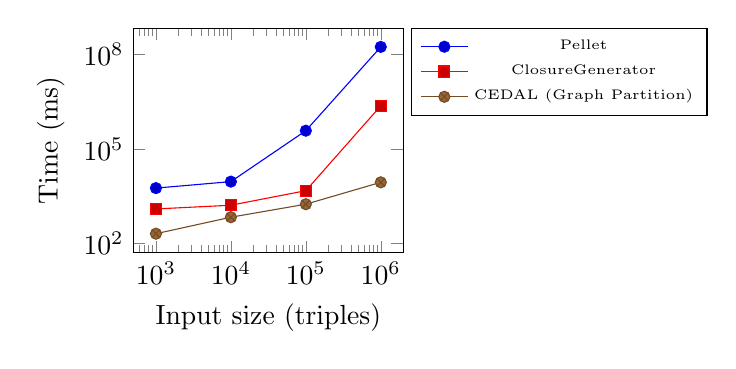
\begin{tikzpicture}
		\begin{axis}[
		scale=0.50,
		ymode = log,
		xmode = log,
		legend style={legend pos=outer north east,font=\tiny},
		xlabel=Input size (triples),
		ylabel=Time (ms)
		]
		\addplot coordinates { % PELLET
			(1000,5635)(10000,9051) (100000,376606) (1000000,173586358)
		};
		\addplot coordinates { % ClosureGenerator
			(1000,1224)(10000,1609) (100000,4663) (1000000,2326869)
		};
		\addplot coordinates { % CEDAL
			(1000,200)(10000,669) (100000,1734) (1000000,8600)
		};
		\legend{
			Pellet,
			ClosureGenerator,
			CEDAL (Graph Partition)
		}
		\end{axis}
		\end{tikzpicture}
	}
	\caption{Pellet vs. ClosureGenerator vs. CEDAL}
	\label{fig:reasoners}
\end{figure}

%\todo[inline]{TS: I think the following paragraph can be omitted.}
%Once we found a way to solve the problem without computing the closures, our problem was reduced to calculating the graph partitions in order to build the clusters that required less computation than closures. Since we did not find a better way using a reasoner to generate the graph partitions, we decided that a reasoner was not required.

%We will not extend to comparisons of graph partitioning, due to the fact that the aim of our work is the quality dimension of conciseness applied to linkset repositories.

%In this section we explain why we choose our own RDF graph partition algorithm instead of use a typical reasoner such as Pellet, since Pellet was considered the best reasoner~\cite{bockbenchmarking} we only compare with him.
%
%As show in figure \ref{fig:reasoners}, we can say that for our aim that is calculate the RDF graph partitions CEDAL outperform Pellet. 
%
%\begin{figure}[] 
%	\begin{tikzpicture}
%	\begin{axis}[
%	scale=0.60,
%	legend style={legend pos=outer north east,font=\tiny},
%	xlabel=Input size (triples),
%	ylabel=Time (ms)
%	]
%	\addplot coordinates { % CEDAL
%		(1000,200)(10000,669) (100000,1734) (1000000,10532) 
%	};
%	\addplot coordinates { % PELLET
%		(1000,1000)(10000,3345) (100000,8670) (1000000,52660) 
%	};
%	\legend{CEDAL,
%		Pellet}
%	\end{axis}
%	\end{tikzpicture}
%	\caption{RDF graph partition CEDAL x Pellet.}
%	\label{fig:reasoners}
%\end{figure}

%\section{Discussion}
%
%At this point we would like to leave two points to discuss, (1) computing the closures and (2) the completeness of LinkLion.
%
%(1) According to~\cite{arenas2008extension}, there is some important points to discuss, for instance, the computation of closures in RDF graph has several drawbacks. First, it is known that the size of the closure of a graph $G$ is of \textbf{quadratic order} in the worst case, making the computation and storage of the closure too expensive for web-scale applications. Second, once the closure has been computed, all queries are evaluated over a data source which can be much larger than the original one. This can be particularly \textbf{inefficient for queries} that must scan a large part of the input data.
%
%%\todo{All this text needs and will be rewrite :)}
%
%(2) The LinkLion approach can be considered almost complete
%i.e., in a single dataset, we can try to discover the transitivity of a given relation because most of the relationships between resources are supposed to exist
%for instance, in LinkLion, we have links from dataset A to B, then B to C, but we cannot assume that links between A and C exist
%it could be that nobody ever tried to discover links from A to C
%so LinkLion does not contain those links. Therefore, we need an approach to generate the Transitive Closure (TC) in this cases.

%\subsection{Potential Applications and use cases}
%LinkLion is our first successful application of our work. Our EDA is applied to a sample of data from LinkLion, but we need the data specialist in order to fix the problem detected by our approach.
